\subsection{Introduction}

Vision Transformers (ViT) apply the self-attention architecture originally
developed for language to images, by splitting an image into a sequence of
fixed-size patches and processing that sequence with the same multi-head
self-attention mechanism used in NLP transformers. Unlike a convolutional
network, whose receptive field grows only gradually with depth through
local, spatially-restricted filters, self-attention lets every patch attend
directly to every other patch from the very first layer -- a fundamentally
different inductive bias with direct consequences for interpretability and
robustness. This section investigates four aspects of a pre-trained ViT:
its zero-shot classification behavior, whether its built-in attention
weights provide a meaningful window into its decision process, how
robustly it tolerates missing input patches under two different masking
strategies, and how the choice of pooling strategy -- the dedicated
classification token versus a simple average of all patch representations
-- affects transfer to a new downstream task.

\subsection{Methodology}

\subsubsection{Model and Preprocessing}

\texttt{google/vit-base-patch16-224}, pretrained on ImageNet, is used
throughout. An input image of $224\times224$ pixels is divided into
non-overlapping $16\times16$ patches, giving
$N=(224/16)^2=196$ patches. Each patch is linearly projected and
concatenated with a learnable classification token (\texttt{[CLS]}) and
positional embeddings, producing a sequence of $197$ tokens fed to $12$
transformer encoder layers.

\subsubsection{Attention Extraction}

Multi-head self-attention computes, for each head $h$ in layer $l$,
\[
  A^{(l,h)} = \mathrm{softmax}\!\left(\frac{QK^\top}{\sqrt{d_k}}\right) \in \mathbb{R}^{197\times197}.
\]
For the final layer, the row corresponding to the \texttt{[CLS]} token
gives its attention to all $196$ patch tokens,
$a^{(h)} = A^{(l=12,h)}_{0,1:197} \in \mathbb{R}^{196}$. This vector is
reshaped to the $14\times14$ patch grid and bilinearly upsampled to
$224\times224$ to produce a heatmap overlay on the original image, for each
of the $12$ heads independently.

\subsubsection{Patch-Masking Protocol}

Two masking strategies are compared at fractions
$f\in\{0,0.1,0.25,0.5,0.75,0.9\}$: \emph{random} masking, which zeroes a
uniformly-random subset of patches (10 independent trials per fraction,
seeds $42$-$51$), and \emph{center} masking, which zeroes a single
deterministic square block of side
$\lceil\sqrt{196f}\rceil$ centered on the $14\times14$ grid. Robustness is
quantified with two metrics: prediction consistency,
\[
  C(f) = \frac{1}{N}\sum_{i=1}^N \mathbb{1}\big[\hat y_i^{(f)} = \hat y_i^{(0)}\big],
\]
and the probability retained on the original predicted class,
\[
  P_{\text{orig}}(f) = \frac{1}{N}\sum_{i=1}^N p_i\big(\hat y_i^{(0)} \mid X_i^{(f)}\big),
\]
where $X_i^{(f)}$ is the masked image and $\hat y_i^{(0)}$ the unmasked
prediction.

\subsubsection{Downstream Probing Setup}

Two pooling strategies are compared as fixed feature extractors for a
linear probe trained on a CIFAR-10 subset (2000 train / 500 test images,
200 images/class): the \texttt{[CLS]} token's final hidden state,
$\mathbf{f}_{\text{CLS}}=\mathbf{h}_{\text{CLS}}=\sum_{j=0}^{N}\mathbf{A}_{0,j}\mathbf{V}_j$,
and the unweighted mean of all 196 patch tokens' final hidden states,
$\mathbf{f}_{\text{mean}}=\frac{1}{N}\sum_{i=1}^{N}\mathbf{z}_i$. The ViT
backbone is kept entirely frozen ($\nabla_{\theta_{\text{ViT}}}=0$); a
single linear head $\mathbf{W}\in\mathbb{R}^{C\times d}$,
$\mathbf{b}\in\mathbb{R}^C$ ($C=10$, $d=768$) is trained on each feature
type by minimizing softmax cross-entropy over the $2000$ training
examples, for $10$ epochs.

\subsection{Results}

\subsubsection{Zero-Shot Classification}

On a test photograph of a leopard, the model's top-5 predictions were:
leopard (0.9900), jaguar (0.0076), cheetah (0.0010), snow leopard (0.0004),
lion (0.0002) -- all five predictions from within the large-cat family.

\subsubsection{Patch Attention Visualization}

\begin{figure}[t]
\centering
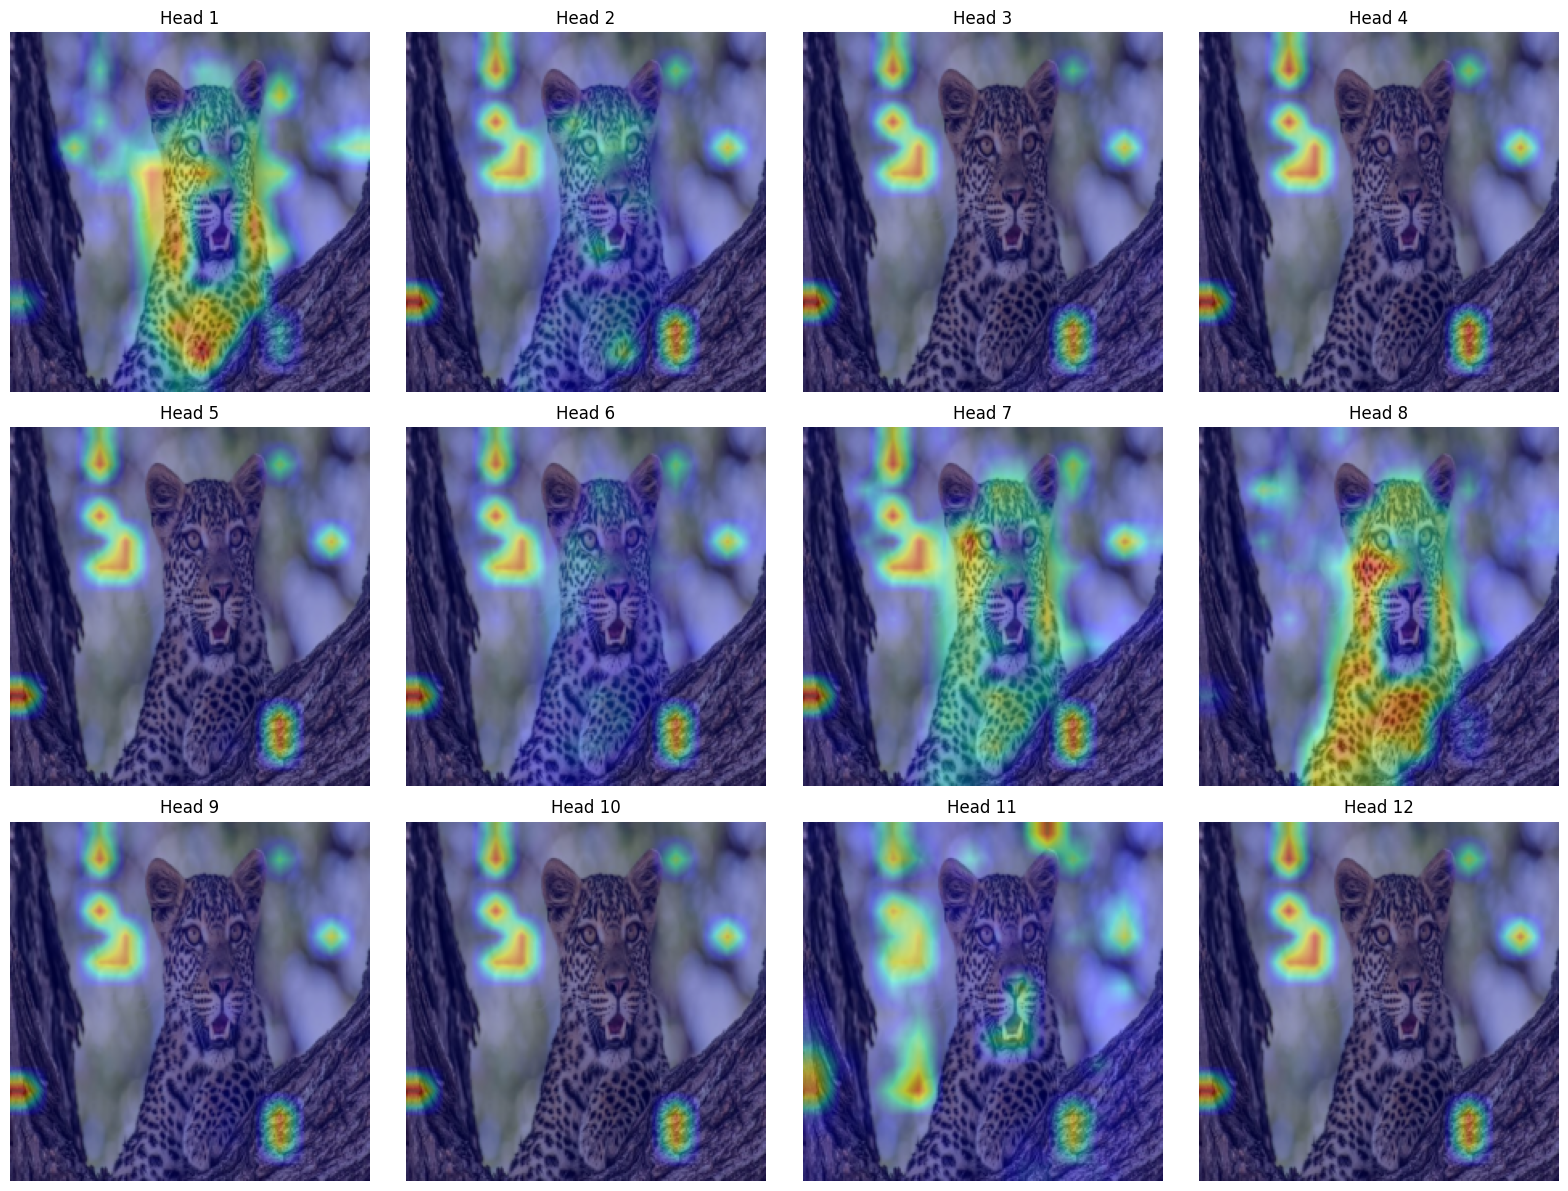
\includegraphics[width=\linewidth]{assets/vit_fig3.png}
\caption{\texttt{[CLS]}-to-patch attention, all 12 heads of the final layer, overlaid on the input image.}
\label{fig:vit-attn}
\end{figure}

Figure~\ref{fig:vit-attn} shows the 12 final-layer attention heads. Heads 1,
7, 8, and 11 concentrate strongly and specifically on the leopard's face
and body; the remaining heads distribute more attention toward background
regions (tree bark, foliage), though at visibly lower intensity than the
four leopard-focused heads.

\subsubsection{Robustness to Patch Masking}
\label{sec:vit-masking-results}

\begin{figure}[t]
\centering
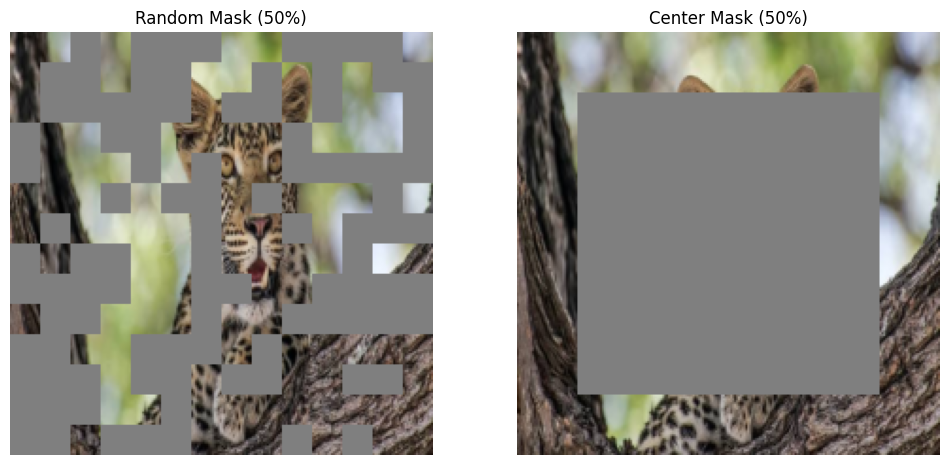
\includegraphics[width=0.9\linewidth]{assets/vit_fig4.png}
\caption{Random vs.\ center masking at $f=0.5$ on the leopard test image.}
\label{fig:vit-mask-example}
\end{figure}

\begin{figure}[t]
\centering
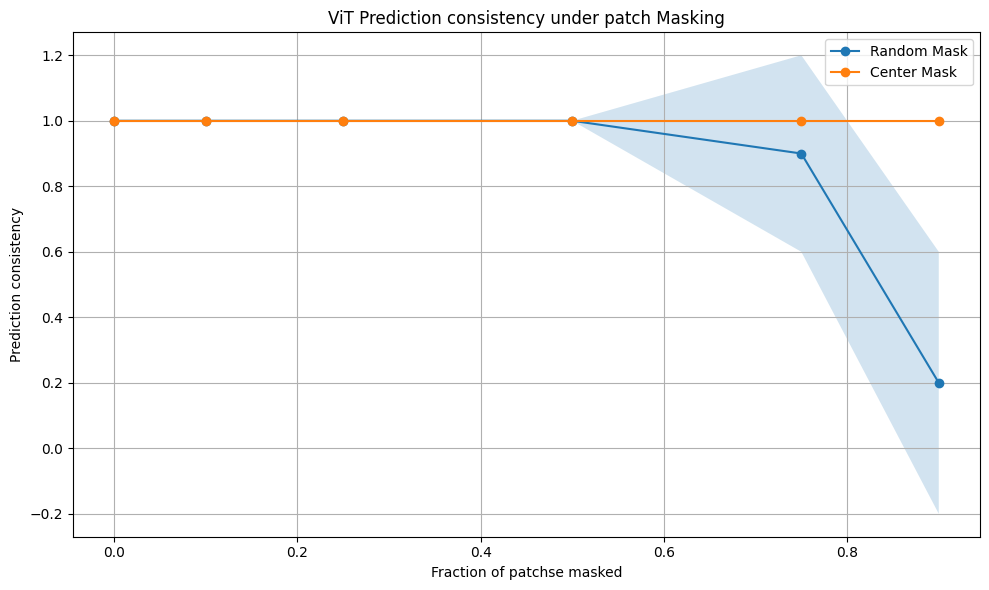
\includegraphics[width=\linewidth]{assets/vit_fig6.png}
\caption{Prediction consistency $C(f)$ vs.\ masking fraction. Shaded band: $\pm 1$ std.\ over 10 random-mask trials; center masking is deterministic (zero variance).}
\label{fig:vit-consistency}
\end{figure}

\begin{figure}[t]
\centering
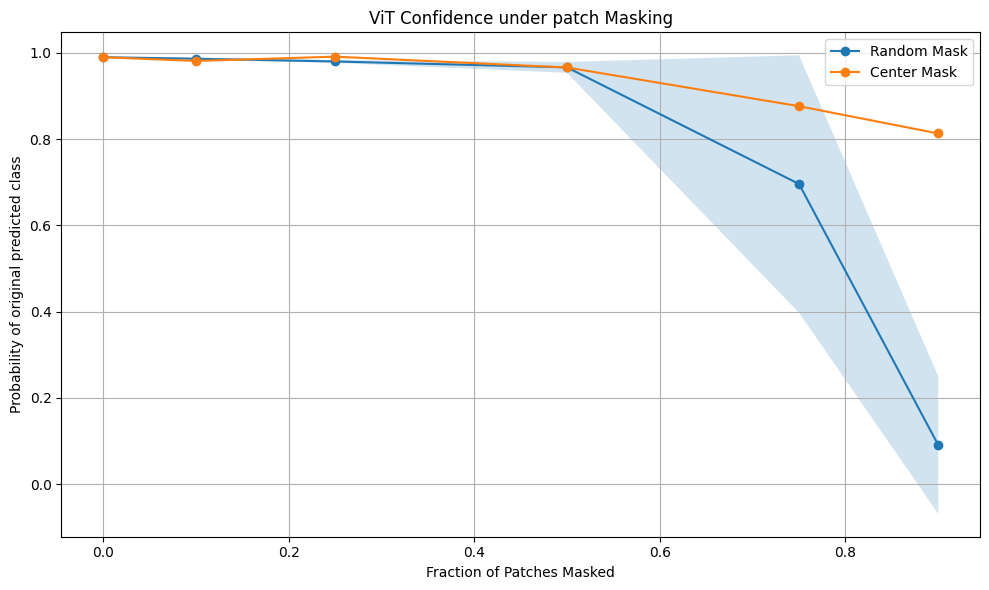
\includegraphics[width=\linewidth]{assets/vit_fig7.png}
\caption{Retained probability of the original predicted class $P_{\text{orig}}(f)$ vs.\ masking fraction.}
\label{fig:vit-confidence}
\end{figure}

Both masking strategies leave $C(f)=1.0$ up to $f=0.5$ (98-100 of 196
patches removed; Figure~\ref{fig:vit-mask-example} shows this level for
both strategies on the test image). Beyond that, the two diverge sharply:
random masking's consistency falls to $0.90\pm0.30$ at $f=0.75$ and
$0.20\pm0.40$ at $f=0.9$, while center masking's consistency remains
exactly $1.0$ at every tested fraction, including $f=0.9$ (169 of 196
patches removed, leaving only a 1-patch-wide border). Confidence in the
original class ($P_{\text{orig}}$) shows the same pattern: random masking
falls to $0.09$ at $f=0.9$, versus $0.81$ for center masking at the same
fraction.

\subsubsection{Downstream Probing}

\begin{figure}[t]
\centering
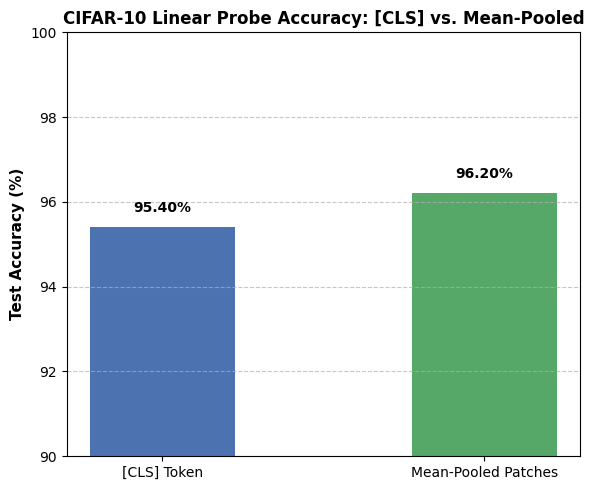
\includegraphics[width=0.8\linewidth]{assets/vit_fig8.png}
\caption{CIFAR-10 linear-probe test accuracy: \texttt{[CLS]} token vs.\ mean-pooled patch tokens.}
\label{fig:vit-probe}
\end{figure}

The mean-pooled probe reaches $96.20\%$ test accuracy, slightly
outperforming the \texttt{[CLS]}-token probe's $95.40\%$ (Figure~\ref{fig:vit-probe}).
Both probes converge to near-perfect training accuracy ($\geq99.5\%$ by
epoch 10), so the $0.8$ percentage-point gap reflects a real, if modest,
generalization difference rather than an undertrained comparison.

\subsection{Discussion}

\subsubsection{Classification Confidence and Fine-Grained Discrimination}

The model assigned $99\%$ probability to the correct \emph{leopard} class,
with all five top predictions drawn from the large-cat family (jaguar,
cheetah, snow leopard, lion). This indicates the model has learned features
general enough to recognize ``large spotted/tawny feline'' robustly, and
specific enough to separate visually similar species within that family --
e.g.\ distinguishing a leopard's rosette-patterned coat from a cheetah's
solid black spots and slimmer build -- rather than merely detecting the
coarse category.

\subsubsection{Attention as Built-in Interpretability vs.\ CAM/Grad-CAM}

The strongest attention regions in several heads overlap with the
leopard's body: if $P$ denotes patches belonging to the leopard and $B$
the background patches, the qualitative pattern observed is
\[
  \sum_{j\in P} a_j \;>\; \sum_{j\in B} a_j,
\]
concentrated particularly in Heads 1, 7, 8, and 11. A larger \emph{number}
of heads distribute some attention to background regions, but at visibly
weaker intensity than these four -- indicating the final layer's
\texttt{[CLS]} representation is shaped predominantly, but not exclusively,
by object-specific evidence.

This attention-based view differs fundamentally from CNN interpretation
methods. \textbf{CAM} constructs a class-specific spatial map from a
convolutional network's final feature maps: for feature map $F_k(x,y)$ and
its learned classifier weight $w_k^c$ for class $c$,
\[
  M_c(x,y) = \sum_k w_k^c F_k(x,y).
\]
\textbf{Grad-CAM} instead weights feature maps by the gradient of the
target class score with respect to their activations,
\[
  \alpha_k^c = \frac{1}{HW}\sum_{x}\sum_{y}\frac{\partial z_c}{\partial F_k(x,y)},
\]
\[
  L^c_{\text{Grad-CAM}} = \mathrm{ReLU}\!\left(\sum_k \alpha_k^c F_k\right).
\]
Both are \emph{post-hoc}: they are computed after a forward (and, for
Grad-CAM, backward) pass through a network that was never designed to
explain itself, reconstructing an approximate explanation from gradients
or learned weights. ViT's attention, by contrast, is a first-class part of
the forward computation that produces the prediction --
$A=\mathrm{softmax}(QK^\top/\sqrt{d_k})$ is literally how information from
each patch is combined at every layer, not an approximation added
afterward. This also means attention naturally exposes \emph{multiple}
independent views (one per head) of what the model is attending to, making
questions about head specialization directly answerable, whereas
CAM/Grad-CAM typically produce a single heatmap per choice of layer.

One caveat is worth stating precisely: built-in attention is still not a
complete causal explanation of the final prediction -- it describes how
representations are weighted and combined at one layer, not the full
multi-layer chain of transformations that produced the logits. CAM/Grad-CAM
and attention visualization should be understood as two different sources
of evidence about a prediction, not as one being strictly superior to the
other.

\subsubsection{Why Center Masking Outperforms Random Masking at Extreme Fractions}

The comparison in Figures~\ref{fig:vit-consistency}-\ref{fig:vit-confidence}
reveals two different \emph{failure modes}, not just two degradation rates.

\textbf{Random masking is governed by chance.} At fraction $f$, $m=N(1-f)$
patches survive, drawn independently and uniformly on each trial. If $D$
denotes the small number of patches carrying the leopard's most
discriminative texture -- consistent with only Heads 1, 7, 8, and 11
concentrating tightly on specific regions rather than the whole animal --
the probability that one random draw misses \emph{every} discriminative
patch follows the hypergeometric tail
\[
  P(\text{no discriminative patch survives}) = \frac{\binom{N-D}{m}}{\binom{N}{m}},
\]
which stays small while $m$ is large and rises sharply once $m$ shrinks
past a threshold relative to $D$ -- exactly the empirical cliff between
$f=0.5$ (consistency $1.0$) and $f=0.9$ (consistency $0.20\pm0.40$). The
large standard deviations at $f=0.75$ ($\pm0.30$) and $f=0.9$ ($\pm0.40$)
are the direct empirical signature: across just 10 seeds, whether the model
still answers correctly is close to a coin flip at extreme masking, since
it depends entirely on which specific patches happened to survive.

\textbf{Center masking is governed by geometry, not chance.} The removed
region is the same deterministic square block regardless of trial -- there
is no randomness to average over, which is why its variance is exactly
zero. Its outcome depends on a single fixed question: does the
always-preserved border ring contain enough discriminative texture? For
this image, evidently yes: consistency stays at $1.0$ even at $f=0.9$
(only a 1-patch-wide border survives), and confidence degrades only to
$0.81$.

\textbf{The mechanistic link back to attention.} This is not a
coincidence: the heads concentrating most strongly on the leopard were
attending to regions distributed across the frame, including areas close
to the image boundary -- exactly what center masking's fixed border
preserves, and exactly what one unlucky random draw can miss entirely. The
core distinction is that random masking's failure reflects one unlucky
sample, not a stable property of the model, while center masking's outcome
is fully determined by where this photograph's discriminative content sits
relative to a fixed region of the frame.

\subsubsection{Pooling Strategy: \texttt{[CLS]} Token vs.\ Mean-Pooled Patches}

The \texttt{[CLS]} token is a \emph{learned}, task-specific aggregator --
during ImageNet pretraining the classification loss was backpropagated
directly through it, so attention was explicitly optimized to route
classification-relevant information into that one token,
$\mathbf{h}_{\text{CLS}}=\sum_{j=0}^{N}\mathbf{A}_{0,j}\mathbf{V}_j$. Mean
pooling, $\mathbf{f}_{\text{mean}}=\frac{1}{N}\sum_{i=1}^{N}\mathbf{z}_i$,
is a fixed, unlearned rule with no such tailoring. A priori this predicts a
\texttt{[CLS]} advantage, but the measured result is the opposite: mean
pooling wins, $96.20\%$ vs.\ $95.40\%$.

The gap is best explained by what each pooling rule discards. The
\texttt{[CLS]} token's attention distribution, as Figure~\ref{fig:vit-attn}
shows directly, is not spread uniformly -- a handful of heads (1, 7, 8, 11)
concentrate sharply on specific high-contrast regions of the object. That
concentration is a feature for the ImageNet objective it was optimized
for, but it also means \texttt{[CLS]} can act as an information
bottleneck: patches outside the heavily-attended regions contribute little
to $\mathbf{h}_{\text{CLS}}$, even if they carry class-relevant evidence.
Mean pooling instead aggregates all $196$ patch tokens uniformly, so no
single patch's information can dominate or be discarded, at the cost of
weighting irrelevant background patches equally with informative ones.

This distinction matters more for CIFAR-10 specifically. Its native
$32\times32$ images are upsampled to $224\times224$ for the pretrained
processor, so central object detail is blurry, and the patch grid encodes a
comparatively coarse, low-frequency version of the scene. Under those
conditions distributed cues -- overall silhouette, background context,
color composition -- carry more of the discriminative signal relative to
fine central detail than they would for a native-resolution ImageNet photo,
which plausibly favors mean pooling's uniform aggregation over
\texttt{[CLS]}'s more selective one. The masking results in
Section~\ref{sec:vit-masking-results} are consistent with this: the model tolerates losing up to
half the patches with zero consistency loss, which only makes sense if
class-relevant evidence here is genuinely distributed across many patches
rather than concentrated in a few -- exactly the regime where averaging
over all patches should not lose much, and where a token that selectively
routes information from a few patches has more to lose.

\textbf{Interaction with the pretraining objective.} The size and even the
sign of this gap should depend on what produced the backbone's weights, not
just on the pooling rule itself. Under \emph{supervised} pretraining (as
used here), the loss is applied directly to \texttt{[CLS]},
$\mathcal{L}_{\text{sup}}=\ell_{\text{CE}}(\mathbf{W}_{\text{head}}\mathbf{h}_{\text{CLS}},y)$,
which forces attention heads to route class-relevant information into that
token specifically -- so both representations end up reasonably
class-discriminative, and the observed gap ($0.8$ points) is small. Under
\emph{masked-autoencoding} pretraining (MAE), which reconstructs raw pixel
values for a large masked fraction via
$\mathcal{L}_{\text{MAE}}=\frac{1}{|\mathcal{M}|}\sum_{i\in\mathcal{M}}\|\hat{\mathbf{x}}_i-\mathbf{x}_i\|_2^2$,
the \texttt{[CLS]} token is never directly supervised at all -- every
patch token instead learns to encode local texture and geometry needed for
reconstruction -- so mean pooling should show a substantially larger
advantage over \texttt{[CLS]} than observed here. Under
\emph{self-distillation} (DINO), where a cross-entropy objective
$\mathcal{L}_{\text{DINO}}=-\sum\mathbf{p}_{\text{teacher}}(\mathbf{h}_{\text{CLS}})\log\mathbf{p}_{\text{student}}(\mathbf{h}_{\text{CLS}})$
aligns \texttt{[CLS]} representations of the same image under different
augmentations, \texttt{[CLS]} is pushed toward capturing high-level,
augmentation-invariant semantic content specifically, which would be
expected to favor \texttt{[CLS]} more than either alternative. The
takeaway is that "which pooling method is better" is not a fixed property
of the ViT architecture -- it is a property of what the backbone's
attention was optimized to route into the \texttt{[CLS]} token during
pretraining, and should be re-evaluated whenever the pretraining objective
changes.
